% Provenance (never printed): see sources/outline_sources.md (Year 3:
% speciation and saturation indices; carbonate equilibria applied to rocks;
% weathering kinetics; hydrothermal fluids). Brief: sources/book5/BRIEFS.md,
% ch. 15. Curves from figdata/bachelor-3/carbonate_system.py,
% activity_diagram.py, weathering_rates.py. Exercise and problem values in the
% Book 5 scratch calculator calc/ch15.py. The spring below the Varden
% limestone, its analysis and the granite stream are invented.
\chapter{Water--gesteenteinteractie}\label{ch:b3:water-rock-interaction}

Een bron aan de voet van een kalksteenescarpement laat op elk twijgje en elke steen die ze raakt een witte korst achter;
een beek die door een graniet stroomt voert silica, natrium
en een beetje kalium af, en laat helemaal geen korst achter. Het verschil zit in de chemie van het water,
en die chemie is een verslag van het gesteente dat het water is gepasseerd: hoeveel koolstofdioxide het meevoerde, hoe lang het er bleef,
welke mineralen het oploste en welke het juist opbouwde. Dit hoofdstuk leest dat verslag met
de hulpmiddelen van de oplossingschemie, van de analyse van een water tot de snelheden van
minerale oplossing en de isotopensporen van hete vloeistoffen
in de korst.

\begin{recall}
Activiteit, activiteitscoëfficiënt, ionsterkte, speciatie, het oplosbaarheidsproduct,
alkaliniteit, de verzadigingstoestand $\Omega$, de wet van Henry, snelheidswetten,
de wet van Arrhenius, de overgangstoestand en de $\delta$-waarde staan in de
universitaire delen van de scheikundeboeken. Chemische verwering, de hydrolyse van
silicaten, kleimineralen en kaoliniet staan in Boek~3, in het hoofdstuk over verwering
en kleien; de lysokline en de carbonaatcompensatiediepte in het hoofdstuk over
carbonaat-, kiezel- en verdampingsgesteenten. De hydrothermale vloeistof staat in Boek~4,
in het hoofdstuk over ertsafzettingen, en de silicaatverweringsthermostaat in het
hoofdstuk over het klimaat in de geologische tijd;
hydrothermale circulatie staat in de schoolboeken.
\end{recall}

\section{De analyse van een natuurlijk water}\label{sec:b3:water-rock-interaction:analysis}

Een wateranalyse geeft de belangrijkste ionen in milligram per liter: calcium,
magnesium, natrium en kalium; bicarbonaat, chloride, sulfaat en nitraat;
opgelost silica als \ce{SiO2}; en de pH en temperatuur gemeten bij de bron,
omdat beide veranderen zodra het monster die bron verlaat. Delen door de molaire massa
geeft millimol per liter, en vermenigvuldigen met de lading milli-equivalenten per liter.
Een verdund water is elektrisch neutraal, dus de som van de kationen moet gelijk zijn
aan de som van de anionen.

\begin{method}[Een wateranalyse controleren]\label{met:b3:water-rock-interaction:analysis}
\begin{enumerate}
\item reken elke concentratie om naar \unit{mmol/L} en naar \unit{meq/L};
\item tel de kationen en de anionen op in \unit{meq/L};
\item bereken de ladingsbalansfout $100\,(\sum\text{cat} -
  \sum\text{an})/(\sum\text{cat} + \sum\text{an})$, in procent;
\item accepteer de analyse als de fout binnen 1 of \qty{2}{\percent} ligt voor een
  water van 250 tot \qty{1000}{mg/L}, iets meer voor een verdunder water;
  zoek anders naar een ontbrekend ion of een analysefout.
\end{enumerate}
\end{method}
% ledger: hem85:charge-balance

De activiteit van een ion is zijn molaliteit maal zijn activiteitscoëfficiënt
$\gamma$. In natuurlijke wateren wordt $\gamma$ berekend uit de ionsterkte $I =
\tfrac12\sum m_i z_i^2$ met de uitgebreide Debye--Hückel-vergelijking
\[
-\log\gamma_i = \frac{A z_i^2\sqrt I}{1 + B a_i\sqrt I},
\]
met $A = 0.5085$ en $B = 0.3281$ voor water bij \qty{25}{\celsius}, en een
ionstraal $a_i$ in ångström: 9 voor \ce{H+}, 8 voor \ce{Mg^2+}, 6 voor
\ce{Ca^2+}, 5 voor \ce{CO3^2-}, 4 voor \ce{Na+}, \ce{HCO3-} en \ce{SO4^2-},
3 voor \ce{K+}, \ce{Cl-}, \ce{OH-} en \ce{NO3-}. De vergelijking geldt tot ongeveer
\qty{0.1}{mol/L} van eenwaardige zouten, wat rivieren en de meeste grondwaters
dekt maar niet zeewater of pekel. Temperatuur verandert $A$ alleen van
0.4883 bij \qty{0}{\celsius} tot 0.5425 bij \qty{60}{\celsius}, dus de waarden bij
\qty{25}{\celsius} gelden ook voor koele wateren.
% ledger: hem85:debye-huckel

De anorganische koolstof van een water is verdeeld over opgelost koolstofdioxide
(geschreven als \ce{CO2} voor de som van \ce{CO2} en \ce{H2CO3}), bicarbonaat en
carbonaat, verbonden door
\[
K_1 = \frac{a_{\ce{HCO3-}}\,a_{\ce{H+}}}{a_{\ce{CO2}}}, \qquad
K_2 = \frac{a_{\ce{CO3^2-}}\,a_{\ce{H+}}}{a_{\ce{HCO3-}}}, \qquad
K_H = \frac{a_{\ce{CO2}}}{P_{\ce{CO2}}},
\]
met $\log K_1 = -6.35$, $\log K_2 = -10.33$ en $\log K_H = -1.47$ bij
\qty{25}{\celsius}, en $-6.46$, $-10.49$ en $-1.27$ bij \qty{10}{\celsius}
($P$ in atmosfeer). Tussen pH 6.4 en 10.3 domineert bicarbonaat, en in de meeste
natuurlijke wateren bestaat de alkaliniteit bijna geheel uit bicarbonaat. Een
gemeten pH en bicarbonaatgehalte geven dan de twee andere species, en de
partiële druk van koolstofdioxide waarmee het water in evenwicht zou zijn.
% ledger: phreeqc:carbonate

\section{Verzadiging}\label{sec:b3:water-rock-interaction:saturation}

\begin{definition}[Verzadigingsindex]\label{def:b3:water-rock-interaction:si}
De \emph{verzadigingsindex (van een mineraal)}\index{verzadigingsindex (van een mineraal)}
in een water is $\mathrm{SI} = \log(\mathrm{IAP}/K)$, waarbij IAP
het ionactiviteitsproduct van het water is, geschreven zoals het oplosbaarheidsproduct
$K$ van het mineraal: $\mathrm{SI} = \log\Omega$.
\end{definition}

Een water met $\mathrm{SI} < 0$ kan het mineraal oplossen, een water met
$\mathrm{SI} > 0$ kan het laten neerslaan, en $\mathrm{SI} = 0$ is evenwicht.
Omdat de vrije energie van de oplossingsreactie $\Delta_r G = RT\ln\Omega
= 2.303\,RT\,\mathrm{SI}$ is, is de verzadigingsindex ook een maat voor de
drijvende kracht, in eenheden van $2.303\,RT$, ongeveer \qty{5.7}{kJ/mol} bij
\qty{25}{\celsius}. Voor calciet geldt $\mathrm{IAP} = a_{\ce{Ca^2+}}
a_{\ce{CO3^2-}}$ en $\log K = -8.45$ bij \qty{25}{\celsius}, $-8.35$ bij
\qty{10}{\celsius}: calciet is in koud water beter oplosbaar. Voor gips geldt $\mathrm{SI} = \log(a_{\ce{Ca^2+}}a_{\ce{SO4^2-}}) + 4.55$;
voor kwarts, waarvan de oplossing neutraal \ce{H4SiO4} geeft, geldt $\mathrm{SI} = \log
a_{\ce{H4SiO4}} + 3.98$, en voor amorf silica is de constante 2.71
in plaats van 3.98. Gemeten indices hebben een onzekerheid van ten minste $\pm0.1$,
en een water binnen $\pm0.3$ van nul wordt beschouwd als dicht bij evenwicht.
% ledger: phreeqc:carbonate, phreeqc:silicates, hem85:si

\section{Carbonaatevenwichten in gesteenten}\label{sec:b3:water-rock-interaction:carbonate}

Calciet lost op in met koolstofdioxide beladen water, volgens
\[
\ce{CaCO3 + CO2 + H2O <=> Ca^2+ + 2 HCO3-},
\qquad K = \frac{a_{\ce{Ca^2+}}\,a_{\ce{HCO3-}}^2}{P_{\ce{CO2}}}
= \frac{K_{\mathrm{cal}}K_1K_H}{K_2},
\]
met $\log K = -5.94$ bij \qty{25}{\celsius} en $-5.59$ bij \qty{10}{\celsius}.
Hoeveel er oplost, hangt af van waar de koolstofdioxide vandaan komt.

\begin{definition}[Open en gesloten carbonaatsystemen]\label{def:b3:water-rock-interaction:open-closed}
Een water lost calciet op in een \emph{open carbonaatsysteem}\index{open carbonaatsysteem}
wanneer het in contact blijft met een gas met een vaste
$P_{\ce{CO2}}$, dat de verbruikte koolstofdioxide aanvult. Dit gebeurt in een
\emph{gesloten carbonaatsysteem}\index{gesloten carbonaatsysteem} wanneer het eerst
met koolstofdioxide is beladen en daarna van het gas is afgesloten, zodat
het enige wat het kan gebruiken de koolstofdioxide is die het bevat.
\end{definition}

\begin{theorem}[Oplosbaarheid van calciet, open en gesloten]\label{thm:b3:water-rock-interaction:calcite}
Voor een water van het calciumbicarbonaattype, met $m$ de molaliteit van calcium,
\[
\text{open:}\quad m = \left(\frac{K\,P_{\ce{CO2}}}{4\gamma_{\ce{Ca^2+}}
\gamma_{\ce{HCO3-}}^2}\right)^{1/3};
\qquad
\text{gesloten:}\quad 4\gamma_{\ce{Ca^2+}}\gamma_{\ce{HCO3-}}^2\,m^3 =
\frac{K_{\mathrm{cal}}K_1}{K_2}\,(C_0 - m),
\]
waarin $C_0 = K_H P_{\ce{CO2}}$ de koolstofdioxide is die is opgenomen voordat het
systeem werd afgesloten.
\end{theorem}

\begin{proof}
Tussen pH 6.5 en 8.5 zijn carbonaat, \ce{H+} en \ce{OH-} verwaarloosbaar naast
bicarbonaat, dus de ladingsbalans is $2m = m_{\ce{HCO3-}}$. Open: $K = \gamma
_{\ce{Ca^2+}}m\,\gamma_{\ce{HCO3-}}^2(2m)^2/P_{\ce{CO2}}$, wat de
derdemachtswortel oplevert. Gesloten: elk opgelost calcium verbruikt één \ce{CO2}, dus $m_{\ce{CO2}}
= C_0 - m$ en $a_{\ce{Ca^2+}}a_{\ce{HCO3-}}^2/a_{\ce{CO2}} = K/K_H =
K_{\mathrm{cal}}K_1/K_2$ geeft de kubische vergelijking.
\end{proof}

In het open systeem groeit het calcium als de derdemachtswortel van $P_{\ce{CO2}}$; in
het gesloten systeem wordt het naar boven begrensd door $C_0$, en de koolstofdioxide die
aan het eind overblijft, en dus de eindwaarde van $P_{\ce{CO2}}$, is veel lager dan aan het begin. Bodemlucht
bevat 10 tot 100 keer zoveel koolstofdioxide als de atmosfeer, gevormd door wortels
en door de afbraak van plantaardig materiaal, en grondwater vertoont meestal
een $P_{\ce{CO2}}$ tussen $10^{-2.5}$ en $10^{-1}$ atmosfeer. Water in contact
met calciet en lucht bevat slechts ongeveer \qty{20}{mg/L} calcium; regenwater dat
via de bodem een kalksteen bereikt, nog open naar het bodemgas, kan
vier of vijf keer zoveel. Karst wordt uitgesleten door deze koolstofdioxide uit de bodem.
% ledger: hem85:pco2, phreeqc:carbonate

De weg terug is ontgassing. Een bron die uit een kalksteen komt, voert
de $P_{\ce{CO2}}$ van de bodem en het gesteente mee, tien tot honderd keer die van
de lucht. Bij contact met de lucht verliest het koolstofdioxide, bicarbonaat wordt
carbonaat, de pH stijgt, en de verzadigingsindex stijgt met meer dan één eenheid,
zoals paneel (b) van de onderstaande figuur laat zien voor de bron uit het
weekendprobleem van dit hoofdstuk.
Calciet slaat neer op de beekbodem en op mossen en twijgjes: tufa van
koude bronnen, travertijn van warme. Bronnen die het gesteente doorlopen
snel, in dagen of weken, via kanalen, bereiken meestal het oppervlak
onderverzadigd; die welke er maandenlang langzaam door sijpelen
komen bijna verzadigd aan de oppervlakte.
% ledger: hem85:pco2, usgsyvo:travertine

\begin{omfigure}
\begin{tikzpicture}
\begin{groupplot}[group style={group size=2 by 1, horizontal sep=1.6cm},
  omrecord, width=0.47\linewidth, height=0.42\linewidth, title style={font=\small},
  tick label style={font=\scriptsize}, label style={font=\small},
  legend style={font=\scriptsize, legend cell align=left}]
\nextgroupplot[title={(a) oplosbaarheid van calciet},
  xlabel={$\log P_{\ce{CO2}}$ (atm)}, ylabel={opgelost calcium (\unit{mmol/L})},
  xmin=-3.5, xmax=-1, ymin=0, ymax=5.5, clip=false,
  xtick={-3.5,-3,-2.5,-2,-1.5,-1}, xticklabels={$-3.5$,$-3$,$-2.5$,$-2$,$-1.5$,$-1$},
  legend style={at={(0.14,0.97)}, anchor=north west}]
\addplot[draw=none, fill=black!6, forget plot] coordinates {(-2.5,0) (-2.5,5.5) (-1,5.5) (-1,0)} -- cycle;
% computed in figdata/bachelor-3/carbonate_system.py
\addplot[omDef, thick] table[x=logp, y=ca_open10] {figdata/out/bachelor-3-carbonate_system-solubility.dat};
\addlegendentry{open, \qty{10}{\celsius}}
\addplot[red!70!black, thick] table[x=logp, y=ca_open25] {figdata/out/bachelor-3-carbonate_system-solubility.dat};
\addlegendentry{open, \qty{25}{\celsius}}
\addplot[omDef, thick, densely dashed] table[x=logp, y=ca_closed10] {figdata/out/bachelor-3-carbonate_system-solubility.dat};
\addlegendentry{gesloten, \qty{10}{\celsius}}
\addplot[red!70!black, thick, densely dashed] table[x=logp, y=ca_closed25] {figdata/out/bachelor-3-carbonate_system-solubility.dat};
\addlegendentry{gesloten, \qty{25}{\celsius}}
\draw[black, densely dotted] (axis cs:-3.37,0) -- (axis cs:-3.37,5.5);
\node[font=\scriptsize, anchor=south] at (axis cs:-3.37,5.5) {lucht};
\node[font=\scriptsize, anchor=north] at (axis cs:-1.4,5.45) {grondwater};
\nextgroupplot[title={(b) ontgassing van de bron},
  xlabel={$\log P_{\ce{CO2}}$ (atm)}, ylabel={SI van calciet},
  xmin=-3.5, xmax=-1.5, ymin=-0.2, ymax=1.9, x dir=reverse, clip=false,
  xtick={-3.5,-3,-2.5,-2,-1.5}, xticklabels={$-3.5$,$-3$,$-2.5$,$-2$,$-1.5$}]
% computed in figdata/bachelor-3/carbonate_system.py
\addplot[omDef, thick] table[x=logp, y=si] {figdata/out/bachelor-3-carbonate_system-degassing.dat};
\addplot[black, densely dotted, domain=-3.5:-1.5, samples=2] {0};
\addplot[red!70!black, only marks, mark=*, mark size=1.6pt] table[x=logp, y=si] {figdata/out/bachelor-3-carbonate_system-ends.dat};
\node[font=\scriptsize, anchor=north west] at (axis cs:-1.84,-0.01) {uitlaat};
\node[font=\scriptsize, anchor=north west] at (axis cs:-3.3,1.55) {lucht};
\end{groupplot}
\end{tikzpicture}

\par\smallskip{\small (a) Calcium dat door water in evenwicht met
calciet is opgelost, uitgezet tegen de partiële druk van koolstofdioxide (voor
het gesloten systeem de druk waarmee het water was beladen): open systeem effen, gesloten
systeem gestreept; koud water lost meer op; de grijze band is het bereik van
grondwater. (b) De bron onder de Varden-kalksteen, bij \qty{10}{\celsius},
die onderweg de heuvel af koolstofdioxide verliest (af te lezen van links naar rechts, op een omgekeerde as)
voordat er calciet ontstaat: het calcium en de alkaliniteit liggen vast, de pH stijgt
van 7.2 naar 8.8, en de verzadigingsindex van 0.04 naar 1.6. De
evenwichtsconstanten komen uit een publieke database, met uitgebreide
Debye--Hückel-activiteitscoëfficiënten.}\label{fig:b3:water-rock-interaction:calcite}
\end{omfigure}
% ledger: phreeqc:carbonate, hem85:debye-huckel, hem85:pco2, data:co2-mlo

Dezelfde chemie, toegepast op de schaal van de oceaan, staat in de
universitaire delen van de scheikundeboeken; de diepte waarop zeewater onderverzadigd raakt
met calciet, de lysokline, en de diepte waaronder calciet zich niet
ophoopt, staan in Boek~3.

\begin{inthefield}[Een bron die zijn eigen terrassen bouwt]
\begin{minipage}[t]{0.52\linewidth}\vspace{0pt}
Bij Palette Spring, een van de Mammoth Hot Springs op het plateau van Yellowstone,
stijgt thermisch water op door een begraven kalksteenlaag en voert die
opgelost mee. Aan het oppervlak
verspreidt het water zich over de eigen afzettingen en verliest koolstofdioxide, en calciumcarbonaat
slaat neer als traveertijn, eerst op de rand van elke poel, waar het water
het dunst is. Geologen die deze bronnen in kaart brengen meten een afzetting van ongeveer
drie millimeter per dag, vijftien keer de snelheid van de tufsteen van koude
bronnen. De oranje en
bruine strepen zijn matten van warmteminnende micro-organismen die in de warme afvoer leven.
\end{minipage}\hfill
\begin{minipage}[t]{0.44\linewidth}\vspace{0pt}
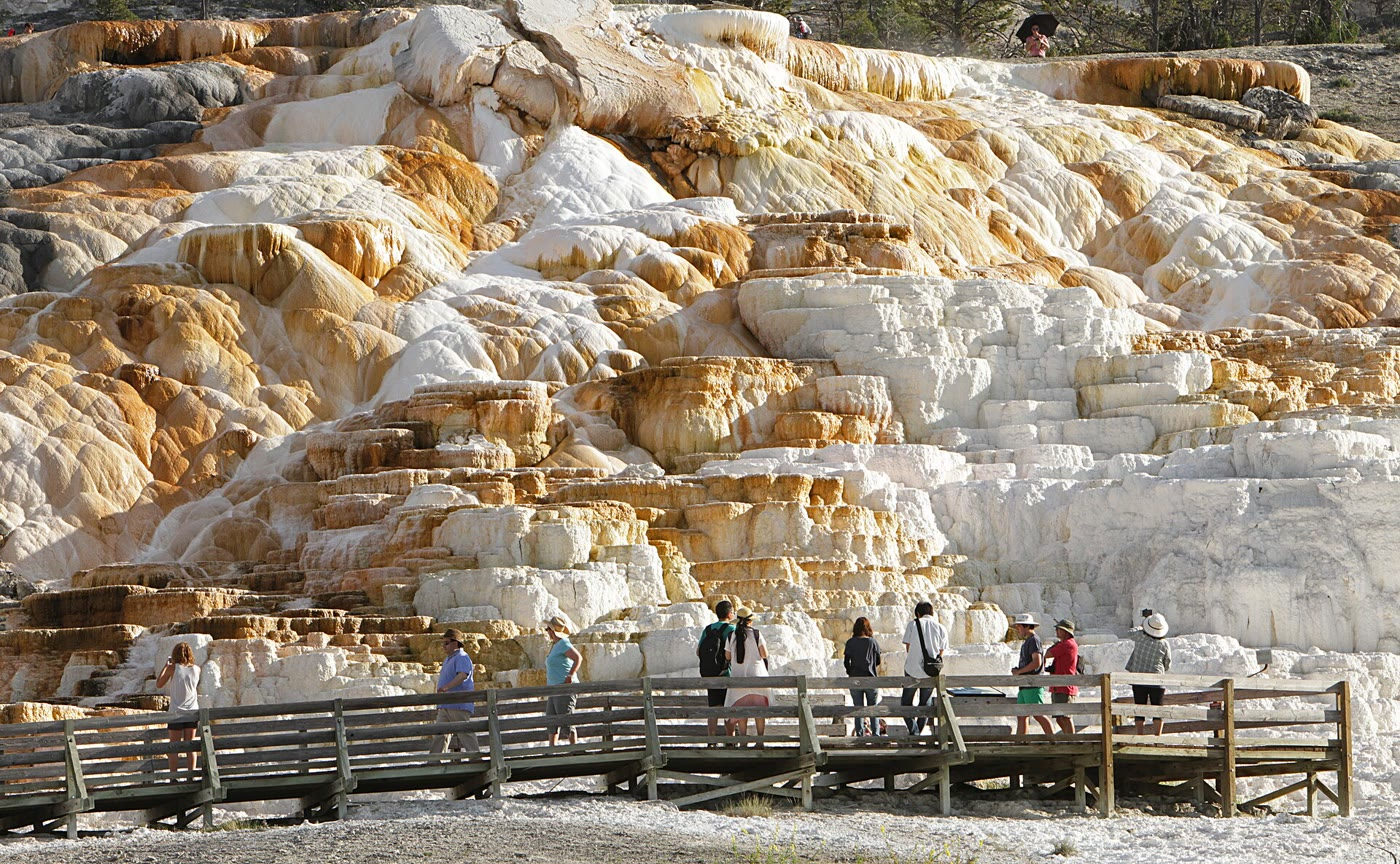
\includegraphics[width=\linewidth]{images/book5/b3-palette-spring-travertine.jpg}

{\scriptsize Traveertijnterrassen van Palette Spring, Mammoth Hot Springs, met
een houten loopbrug en bezoekers ter schaal. NPS-foto door Jim Peaco, publiek domein.}
\end{minipage}
\end{inthefield}
% ledger: photo:b3-palette-spring, usgsyvo:travertine, nps:travertine-terraces

\section{Kinetiek van silicaatverwering}\label{sec:b3:water-rock-interaction:kinetics}

Silicaten lossen veel trager op dan calciet, en een water bereikt zelden
evenwicht met ze: hun oplossing moet met een snelheid worden beschreven.

\begin{definition}[Snelheidswet van minerale oplossing]\label{def:b3:water-rock-interaction:rate-law}
De \emph{snelheidswet van minerale oplossing}\index{snelheidswet van minerale oplossing}
geeft de snelheid van oplossing per eenheid van mineraaloppervlak, in
\unit{mol.m^{-2}.s^{-1}}, als som over zure, neutrale en basische mechanismen,
\[
r = \sum_j k_j\,e^{-\frac{E_j}{R}\left(\frac1T - \frac1{298.15}\right)}\,
a_{\ce{H+}}^{n_j}\,\bigl(1 - \Omega^{p_j}\bigr)^{q_j},
\]
met snelheidsconstanten $k_j$ bij \qty{25}{\celsius}, activeringsenergieën $E_j$,
reactieordes $n_j$ (negatief voor het basische mechanisme) en twee exponenten
$p_j$, $q_j$, die gewoonlijk gelijk aan 1 worden genomen.
\end{definition}
% ledger: pk04:rate-law

\begin{proposition}[Ver van en dicht bij evenwicht]\label{prop:b3:water-rock-interaction:affinity}
Met $p = q = 1$ hangt de snelheid niet af van de verzadiging van het water
wanneer $\Omega \ll 1$, en dicht bij evenwicht is zij evenredig met de
verzadigingsindex: $r \approx -2.303\,r_\infty\,\mathrm{SI}$, waarbij
$r_\infty$ de snelheid ver van evenwicht is.
\end{proposition}

\begin{proof}
De factor is $1 - \Omega = 1 - 10^{\mathrm{SI}}$. Voor $\mathrm{SI} \ll 0$ nadert
hij 1; voor $\mathrm{SI}$ dicht bij 0 geldt $10^{\mathrm{SI}} \approx 1 +
2.303\,\mathrm{SI}$.
\end{proof}

De snelheidsconstanten komen uit laboratoriumexperimenten op verse mineraalpoeders,
in doorstroomreactoren die ver van evenwicht worden gehouden. De figuur hieronder tekent
de snelheidswet voor vier mineralen bij \qty{25}{\celsius}. Elke kromme is een V of een
U: protonen versnellen de oplossing in zuur water, hydroxide in basisch water, en in
daartussen legt het neutrale mechanisme een ondergrens vast. Olivijn lost ongeveer drie
ordes van grootte sneller op dan albiet bij pH~5, waarom het het eerste is van
de gewone silicaten dat uit een bodem verdwijnt. De activeringsenergieën van
albiet en forsteriet, 65 tot \qty{79}{kJ/mol}, maken hun snelheden vier tot vijf
keer hoger bij \qty{25}{\celsius} dan bij \qty{10}{\celsius}.
% ledger: pk04:rates

Veldsnelheden liggen lager, met ordes van grootte. In kolomexperimenten op
vers gebroken graniet daalde de snelheid van plagioklaas gestaag over zes jaar
tot \qty{7.0e-14}{mol.m^{-2}.s^{-1}}; hetzelfde graniet, natuurlijk verweerd,
en deels omgezet tot kaoliniet, loste op met \qty{2.1e-15}{mol.m^{-2}.s^{-1}}
onder dezelfde omstandigheden, en beide zijn nog veel sneller dan de snelheid
die in het verweringsprofiel zelf is gemeten. Over vele mineralen en ouderdommen daalt de
snelheid met de tijd $t$ dat het mineraal heeft verweerd als $R =
\num{3.1e-13}\,t^{-0.61}$ (mol\,m$^{-2}$\,s$^{-1}$, $t$ in jaar). Een deel van
de daling zit in het mineraal, waarvan de meest reactieve oppervlakken het eerst oplossen;
de rest zit in de omgeving: traag water, veel mineraal voor weinig vloeistof, en
poriewater dicht bij evenwicht, waar de bovenstaande propositie de snelheid
klein maakt.
% ledger: whitebrantley03:rates

\begin{omfigure}
\begin{tikzpicture}
\begin{axis}[omrecord, width=0.74\linewidth, height=0.46\linewidth,
  xlabel={pH}, ylabel={$\log r$ (\unit{mol.m^{-2}.s^{-1}})},
  xmin=0, xmax=14, ymin=-14.5, ymax=-6, clip=false,
  xtick={0,2,4,6,8,10,12,14}, ytick={-14,-12,-10,-8,-6},
  yticklabels={$-14$,$-12$,$-10$,$-8$,$-6$},
  tick label style={font=\scriptsize}, label style={font=\small},
  legend style={font=\scriptsize, legend cell align=left, at={(1.03,0.5)}, anchor=west}]
% computed in figdata/bachelor-3/weathering_rates.py
\addplot[green!45!black, thick] table[x=ph, y=forsterite] {figdata/out/bachelor-3-weathering_rates-curves.dat};
\addlegendentry{forsteriet}
\addplot[omDef, thick] table[x=ph, y=albite] {figdata/out/bachelor-3-weathering_rates-curves.dat};
\addlegendentry{albiet}
\addplot[red!70!black, thick, densely dashed] table[x=ph, y=kfeldspar] {figdata/out/bachelor-3-weathering_rates-curves.dat};
\addlegendentry{K-veldspaat}
\addplot[black, thick, densely dotted] table[x=ph, y=kaolinite] {figdata/out/bachelor-3-weathering_rates-curves.dat};
\addlegendentry{kaoliniet}
\end{axis}
\end{tikzpicture}

\par\smallskip{\small Oplossingssnelheden ver van evenwicht bij
\qty{25}{\celsius}, uitgezet tegen de pH, uit een gepubliceerde compilatie van
laboratoriumsnelheidsparameters. Het olivijn-eindlid forsteriet heeft geen basisch mechanisme in
de compilatie; de kromme daalt niet verder dan de neutrale ondergrens.}\label{fig:b3:water-rock-interaction:rates}
\end{omfigure}
% ledger: pk04:rates

\begin{definition}[Verweringsregimes]\label{def:b3:water-rock-interaction:regimes}
Chemische verwering in een landschap bevindt zich in een \emph{aanvoerbeperkt
regime}\index{aanvoerbeperkt regime} wanneer ze wordt begrensd door de snelheid waarmee
erosie verse mineralen naar het verweringsfront brengt, en in een
\emph{verweringsbeperkt regime}\index{verweringsbeperkt regime} wanneer verse
mineralen ruim aanwezig zijn en de snelheid van de reacties haar begrenst.
\end{definition}

Een compilatie van kleine stroomgebieden toont beide. Waar erosie traag verloopt,
onder dikke en uitgeloogde bodems op zacht reliëf, volgt de verweringsflux de
erosiesnelheid: al het verse gesteente dat aankomt, wordt volledig uitgeloogd, en
een warmer of natter klimaat verandert weinig. Waar erosie snel verloopt, in steile
bergen, neemt de flux toe met de afvoer, als de wortel van de erosiesnelheid, en met
de temperatuur, met een schijnbare activeringsenergie van $74 \pm
\qty{29}{kJ/mol}$. Alleen in het tweede regime kan silicaatverwering
fungeren als de klimaatthermostaat van Boek~4.
% ledger: west05:regimes

Welk secundair mineraal een verweringswater vormt, wordt afgelezen uit een ander
diagram.

\begin{definition}[Activiteitsdiagram]\label{def:b3:water-rock-interaction:activity-diagram}
Een \emph{activiteitsdiagram (mineraalstabiliteit)}\index{activiteitsdiagram (mineraalstabiliteit)}
verdeelt een vlak van activiteitsverhoudingen van een water, zoals
$\log(a_{\ce{K+}}/a_{\ce{H+}})$ uitgezet tegen $\log a_{\ce{H4SiO4}}$, in de
velden waarin elk mineraal van een chemisch systeem het stabiele is.
\end{definition}

\begin{proposition}[Grenzen van een activiteitsdiagram]\label{prop:b3:water-rock-interaction:boundaries}
In het systeem \ce{K2O}--\ce{Al2O3}--\ce{SiO2}--\ce{H2O}, met aluminium behouden in de
vaste fasen en water met eenheidsactiviteit, legt een mineraal met $k$ kalium-,
$a$ aluminium- en $s$ siliciumatomen per formule-eenheid en een oplossingsconstante $K$
(naar \ce{K+}, \ce{Al^3+}, \ce{H4SiO4}) vast
\[
\log\frac{a_{\ce{Al^3+}}}{a_{\ce{H+}}^3} = \frac{\log K - kX - sY}{a},
\qquad X = \log\frac{a_{\ce{K+}}}{a_{\ce{H+}}},\quad Y = \log a_{\ce{H4SiO4}}.
\]
Het stabiele mineraal geeft de laagste aluminiumactiviteit, en de grens
tussen twee mineralen is een rechte lijn in $(Y, X)$.
\end{proposition}

\begin{proof}
De oplossing verbruikt $h = k + 3a$ protonen, volgens de ladingsbalans, dus $a\log
a_{\ce{Al^3+}} = \log K + h\log a_{\ce{H+}} - k\log a_{\ce{K+}} - s\log
a_{\ce{H4SiO4}}$; delen door $a$ en $3\log a_{\ce{H+}}$ naar links brengen
geeft de uitdrukking. Een water in evenwicht met één mineraal is
onderverzadigd ten opzichte van elk mineraal dat meer aluminium nodig zou hebben, en
oververzadigd ten opzichte van elk mineraal dat er minder nodig zou hebben, dus het minst
oplosbare mineraal is het stabiele. Gelijkstellen van twee zulke uitdrukkingen, lineair in $X$ en $Y$, geeft een lijn.
\end{proof}

Bij de constanten bij \qty{25}{\celsius} maakt gibbsiet plaats voor kaoliniet bij
$\log a_{\ce{H4SiO4}} = -4.39$ (\qty{2.4}{mg/L} aan silica) en kaoliniet maakt plaats voor
muscoviet bij $\log(a_{\ce{K+}}/a_{\ce{H+}}) = 1.55$, en K-veldspaat is
alleen stabiel in wateren die rijk zijn aan kalium en silica. Het diagram is de verweringsreeks van
Boek~3 in getallen: een verdund water dat kalium en silica wegspoelt, ontdoet een
veldspaat tot gibbsiet; een water dat meer silica behoudt, maakt kaoliniet; een water
dat meer kalium behoudt, zoals op diepte,
maakt een mica.
% ledger: phreeqc:silicates

\begin{omfigure}
\begin{tikzpicture}
\begin{axis}[omrecord, width=0.66\linewidth, height=0.5\linewidth,
  xlabel={$\log a_{\ce{H4SiO4}}$}, ylabel={$\log(a_{\ce{K+}}/a_{\ce{H+}})$},
  xmin=-6, xmax=-2, ymin=0, ymax=10, clip=false,
  xtick={-6,-5,-4,-3,-2}, xticklabels={$-6$,$-5$,$-4$,$-3$,$-2$},
  tick label style={font=\scriptsize}, label style={font=\small}]
% computed in figdata/bachelor-3/activity_diagram.py
\addplot[black, thick, unbounded coords=jump] table[x=y, y=x] {figdata/out/bachelor-3-activity_diagram-lines.dat};
\addplot[omDef, densely dashed] table[x=y, y=x] {figdata/out/bachelor-3-activity_diagram-quartz.dat};
\addplot[omDef, densely dotted] table[x=y, y=x] {figdata/out/bachelor-3-activity_diagram-amorph.dat};
\addplot[red!70!black, only marks, mark=*, mark size=1.8pt] table[x=y, y=x] {figdata/out/bachelor-3-activity_diagram-samples.dat};
\node[font=\small] at (axis cs:-5.4,0.8) {gibbsiet};
\node[font=\small] at (axis cs:-3.25,0.75) {kaoliniet};
\node[font=\small] at (axis cs:-4.6,5.0) {muscoviet};
\node[font=\small] at (axis cs:-3.3,9.3) {K-veldspaat};
\node[font=\scriptsize, omDef, anchor=south] at (axis cs:-3.98,10) {kwarts};
\node[font=\scriptsize, omDef, anchor=south] at (axis cs:-2.71,10) {amorf silica};
\node[font=\scriptsize, red!70!black, anchor=west] at (axis cs:-4.58,0.38) {A};
\node[font=\scriptsize, red!70!black, anchor=west] at (axis cs:-3.80,1.29) {B};
\node[font=\scriptsize, red!70!black, anchor=west] at (axis cs:-3.48,4.08) {C};
\end{axis}
\end{tikzpicture}

\par\smallskip{\small Stabiliteitsvelden in het systeem
\ce{K2O}--\ce{Al2O3}--\ce{SiO2}--\ce{H2O} bij \qty{25}{\celsius}, met de verzadiging van kwarts
(gestreept) en amorf silica (gestippeld). Drie verzonnen wateren: A, een verdunde
tropische beek; B, een beek op graniet; C, een diep grondwater in
graniet.}\label{fig:b3:water-rock-interaction:activity}
\end{omfigure}
% ledger: phreeqc:silicates

\section{Hydrothermale vloeistoffen}\label{sec:b3:water-rock-interaction:hydrothermal}

Heet water dat door de korst circuleert, nabij een rug of een intrusie,
wisselt zuurstof uit met het gesteente dat het doorkruist. Bij hoge temperatuur is de
fractionering tussen gesteente en water klein, en beide bewegen naar
isotopenevenwicht: meteorisch water, licht, maakt het gesteente lichter, en het
water zwaarder. Hoe ver het gesteente is verschoven, meet hoeveel water er
is gepasseerd.

\begin{definition}[Water--gesteenteverhouding]\label{def:b3:water-rock-interaction:water-rock-ratio}
De \emph{water--gesteenteverhouding}\index{water--gesteenteverhouding} $W/R$ van een
hydrothermisch systeem is de massa water die met een massa gesteente is uitgewisseld,
gedeeld door die massa gesteente.
\end{definition}

\begin{proposition}[Water--gesteenteverhoudingen uit zuurstofisotopen]\label{prop:b3:water-rock-interaction:wr}
Laat een gesteente met beginwaarde $\delta_r^i$ zuurstof uitwisselen met een water met
beginwaarde $\delta_w^i$ totdat het $\delta_r^f$ bereikt, in evenwicht met het water
waarmee het laatst in contact kwam, $\Delta = \delta_r^f - \delta_w^f$, en $c_r$ en $c_w$ de
zuurstofconcentraties van gesteente en water zijn. In een gesloten systeem (één
portie water) en in een open systeem (water dat eenmalig passeert),
\[
\frac WR\Big|_{\text{gesloten}} = \frac{c_r}{c_w}\,
\frac{\delta_r^f - \delta_r^i}{\delta_w^i - \delta_r^f + \Delta},
\qquad
\frac WR\Big|_{\text{open}} = \frac{c_r}{c_w}\,
\ln\!\left(\frac{\delta_r^f - \delta_r^i}{\delta_w^i - \delta_r^f + \Delta} + 1\right).
\]
\end{proposition}

\begin{proof}
Gesloten: zuurstof-18 blijft behouden, $c_wW\delta_w^i + c_rR\delta_r^i = c_wW
\delta_w^f + c_rR\delta_r^f$, met $\delta_w^f = \delta_r^f - \Delta$; los
$W/R$ op. Open: een portie $\mathrm dW$ stroomt binnen bij $\delta_w^i$ en verlaat
in evenwicht met het gesteente, bij $\delta_r - \Delta$, zodat $c_rR\,\mathrm d\delta_r
= c_w(\delta_w^i - \delta_r + \Delta)\,\mathrm dW$. Na scheiding,
$\int_{\delta_r^i}^{\delta_r^f}\mathrm d\delta_r/(\delta_w^i - \delta_r +
\Delta) = (c_w/c_r)\,W/R$, en de integraal is $-\ln[(\delta_w^i - \delta_r^f
+ \Delta)/(\delta_w^i - \delta_r^i + \Delta)]$, wat de uitdrukking is.
\end{proof}

Voor zuurstof ligt $c_r/c_w$ dicht bij 0.5. Het open systeem heeft altijd minder
water nodig dan het gesloten systeem bij dezelfde verschuiving, omdat elke portie
zo zwaar mogelijk weggaat. Rond veel intrusies tekent de $\delta^{18}\mathrm O$ van het
nevengesteente een schietschijf van lage waarden, van ongeveer $+6$ tot onder
0, gecentreerd waar het meeste water passeerde; de ertsen van de hydrothermale
vloeistof liggen vaak binnen de laagste contour, waardoor de kaart een
exploratiehulpmiddel is.
% ledger: white13c9:water-rock

\begin{omfigure}
\begin{tikzpicture}[font=\small, >=Stealth]
\draw[thick, fill=black!6] (0,0) rectangle (4,2.2);
\node at (2,1.55) {gesteente, massa $R$};
\node at (2,0.95) {$\delta_r^i \to \delta_r^f$};
\node[font=\scriptsize] at (2,0.4) {uitwisseling bij $T$};
\draw[->, thick, omDef] (-2.6,1.1) -- (-0.1,1.1);
\node[omDef, anchor=south, align=center, font=\scriptsize] at (-1.35,1.15) {water in\\ $\delta_w^i$, $\mathrm dW$};
\draw[->, thick, red!70!black] (4.1,1.1) -- (6.6,1.1);
\node[red!70!black, anchor=south, align=center, font=\scriptsize] at (5.35,1.15) {water uit\\ $\delta_r - \Delta$};
\node[anchor=north, font=\scriptsize, align=center] at (2,-0.15) {open systeem: elke portie passeert eenmaal en verlaat in\\ evenwicht met het gesteente waarmee het laatst in contact kwam};
\end{tikzpicture}

\par\smallskip{\small Het doosmodel van een hydrothermisch systeem. In een gesloten
systeem blijft één portie water bij het gesteente tot beide in evenwicht zijn;
in een open systeem stroomt het water door, en het gesteente verschuift met elke portie
een beetje naar het water toe.}\label{fig:b3:water-rock-interaction:box}
\end{omfigure}

\begin{definition}[Reactiepadmodel]\label{def:b3:water-rock-interaction:reaction-path}
Een \emph{reactiepadmodel}\index{reactiepadmodel} volgt de
samenstelling van een water en de mineralen die het vormt naarmate een reactie vordert,
door kleine hoeveelheden van een reactant toe te voegen (een mineraal dat oplost, een gas dat ontsnapt,
warmte afgevoerd) en bij elke stap de speciatie en de verzadigingsindices opnieuw berekent,
elke stap, waarbij elk mineraal dat verzadiging bereikt neerslaat.
\end{definition}

Een \omterm{def:b3:water-rock-interaction:reaction-path}{reactiepadmodel} dat op de bron van het weekendprobleem draait, waarbij
stap voor stap ontgast wordt, slaat calciet neer zodra de index boven nul komt; gedraaid op
een graniet en een regenwater, vormt het eerst gibbsiet, dan kaoliniet, dan
mica naarmate het water silica en kalium opneemt, en volgt zo een pad over het
activiteitsdiagram. Speciatieprogramma's doen dit met databanken van evenwichtsconstanten
zoals die in dit hoofdstuk worden gebruikt.
% ledger: phreeqc:silicates

\section{Oefeningen}

\begin{exercise}[$\star$]\label{exo:b3:water-rock-interaction:1}
Een water bevat (in \unit{mg/L}) \ce{Ca} 48, \ce{Mg} 9.7, \ce{Na} 23, \ce{K} 3.9,
\ce{HCO3} 183, \ce{Cl} 35.5 en \ce{SO4} 48. Bereken de
ladingsbalansfout. Is de analyse acceptabel?
\end{exercise}

\begin{exercise}[$\star$]\label{exo:b3:water-rock-interaction:2}
Bereken bij een ionsterkte van 0.0050 de activiteitscoëfficiënten van
\ce{Ca^2+}, \ce{HCO3-} en \ce{SO4^2-}.
\end{exercise}

\begin{exercise}[$\star$]\label{exo:b3:water-rock-interaction:3}
Een water dat door een gipshoudende mergel sijpelt, bevat \qty{3.0}{mmol/L} calcium en
\qty{4.0}{mmol/L} sulfaat, bij een ionsterkte van 0.016. Bereken de
verzadigingsindex van gips. Kan het water nog gips oplossen?
\end{exercise}

\begin{exercise}[$\star$]\label{exo:b3:water-rock-interaction:4}
Een grondwater bevat \qty{12}{mg/L} silica, uitgedrukt als \ce{SiO2} en
aanwezig als \ce{H4SiO4}. Bereken de verzadigingsindices voor kwarts en voor
amorf silica bij \qty{25}{\celsius}.
\end{exercise}
% ledger: phreeqc:silicates

\begin{exercise}[$\star\star$]\label{exo:b3:water-rock-interaction:5}
Neem activiteitscoëfficiënten gelijk aan 1 en bereken het calcium dat
een open systeem oplost bij $P_{\ce{CO2}} = 10^{-2}$~atm, bij \qty{25}{\celsius} en bij
\qty{10}{\celsius}, in \unit{mmol/L} en \unit{mg/L}.
\end{exercise}

\begin{exercise}[$\star\star$]\label{exo:b3:water-rock-interaction:6}
Een water bij \qty{25}{\celsius} heeft pH 7.60 en \qty{4.0}{mmol/L}
bicarbonaat. Neem activiteitscoëfficiënten van 1 en bereken het opgeloste
koolstofdioxide en carbonaat, de $P_{\ce{CO2}}$ en het aandeel van elke soort in
het opgeloste anorganische koolstof.
\end{exercise}

\begin{exercise}[$\star\star$]\label{exo:b3:water-rock-interaction:7}
Een albietkorrel is een bol van \qty{1}{mm} doorsnede in een bodemwater van pH 5 bij
\qty{25}{\celsius}, die oplost met de snelheid uit de figuur, $\log r = -12.09$.
Met een molair volume van \qty{101.31}{cm^3/mol}, hoe snel krimpt de straal
ervan, en hoe lang duurt het?
\end{exercise}
% ledger: pk04:rates, phreeqc:silicates

\begin{exercise}[$\star\star$]\label{exo:b3:water-rock-interaction:8}
Met welke factor neemt de neutrale oplossingssnelheid van albiet toe ($E =
\qty{69.8}{kJ/mol}$) van \qty{5}{\celsius} tot \qty{25}{\celsius}? En
een verweringsflux met $E = \qty{74}{kJ/mol}$?
\end{exercise}
% ledger: pk04:rates, west05:regimes

\begin{exercise}[$\star\star$]\label{exo:b3:water-rock-interaction:9}
Leid de kaoliniet--muscoviet-grens van het activiteitsdiagram af uit de
constanten $\log K = 7.435$ (kaoliniet, 2 Al, 2 Si) en $12.703$ (muscoviet, 1
K, 3 Al, 3 Si). Een water bij \qty{25}{\celsius} heeft \qty{2.0}{mg/L}
kalium, \qty{15}{mg/L} silica en pH 7.0: welk mineraal vormt het?
\end{exercise}
% ledger: phreeqc:silicates

\begin{exercise}[$\star\star\star$]\label{exo:b3:water-rock-interaction:10}
Nabij een intrusie wordt een granodioriet van $\delta^{18}\mathrm O = +6$ aangetroffen
bij $-2$ (\unit{\permil}). Het meteorische water had $-13$, en bij de
uitwisselingstemperatuur was het gesteente \qty{2}{\permil} zwaarder dan het
water. Met $c_r/c_w = 0.5$ bereken je niet; bereken de \omterm{def:b3:water-rock-interaction:water-rock-ratio}{water--gesteenteverhouding} voor een gesloten en
een open systeem, en verklaar waarom ze verschillen.
\end{exercise}
% ledger: white13c9:water-rock

\begin{exercise}[$\star\star\star$]\label{exo:b3:water-rock-interaction:11}
Regen beladen met bodemgas, met $P_{\ce{CO2}} = 10^{-1.5}$~atm bij
\qty{10}{\celsius} bereikt een kalksteen. Met activiteitscoëfficiënten gelijk aan 1
bereken het calcium dat het oplost als het open blijft staan voor het bodemgas en als het
eerst van dat gas is geïsoleerd. Welk deel van zijn koolstofdioxide blijft over in het
gesloten geval, en wat is de uiteindelijke $P_{\ce{CO2}}$?
\end{exercise}

\begin{exercise}[$\star\star\star$]\label{exo:b3:water-rock-interaction:12}
Gebruik de propositie over snelheden nabij evenwicht. Welk deel van de
snelheid ver van evenwicht lost een mineraal op bij $\mathrm{SI} =
-2$, $-1$ en $-0.1$? Een laboratoriumsnelheid, gemeten na 6 jaar reactie,
volgt de machtswet uit het hoofdstuk: met welke factor zal ze gedaald zijn
na \num{10000} jaar? Combineer beide effecten om te verklaren waarom veldsnelheden
zo laag zijn.
\end{exercise}
% ledger: whitebrantley03:rates

\section{Probleem: De bron onder de Varden-kalksteen}

\begin{problem}[{Weekendprobleem --- de analyse, koolstofdioxide en
verzadiging van een verzonnen kalksteenbron, en een granietbeek}]
\label{pb:b3:water-rock-interaction:1}
Een bron ontspringt aan de voet van de Jurassische kalksteen van de Varden Hills, bij
\qty{10}{\celsius} en pH 7.20. De analyse ervan is (in \unit{mg/L}): \ce{Ca}
112, \ce{Mg} 4.0, \ce{Na} 7.0, \ce{K} 1.2, \ce{HCO3} 340, \ce{Cl} 11,
\ce{SO4} 14, \ce{NO3} 9. Bij \qty{10}{\celsius}: $\log K_{\mathrm{cal}} =
-8.35$, $\log K_1 = -6.46$, $\log K_2 = -10.49$, $\log K_H = -1.27$. Gebruik de
uitgebreide Debye--Hückel-vergelijking uit het hoofdstuk, negeer ionparen, en neem
de lucht bij $\log P_{\ce{CO2}} = -3.37$.

\medskip\noindent\textbf{Deel I --- De analyse.}
\begin{enumerate}
\item Reken de analyse om naar \unit{mmol/L}.
\item Bereken de ladingsbalansfout. Is de analyse aanvaardbaar?
\item Bereken de ionsterkte.
\item Bereken de activiteitscoëfficiënten van \ce{Ca^2+}, \ce{HCO3-} en
  \ce{CO3^2-}.
\item Is de uitgebreide Debye--Hückel-vergelijking hier geldig?
\end{enumerate}

\medskip\noindent\textbf{Deel II --- Koolstofdioxide.}
\begin{enumerate}[resume]
\item Bereken de activiteit van waterstofcarbonaat.
\item Bereken de activiteit van opgelost koolstofdioxide.
\item Bereken de $P_{\ce{CO2}}$ van de bron. Hoeveel keer die van de
  lucht is dat, en waar kan het koolstofdioxide vandaan komen?
\item Bereken de carbonaatconcentratie en het aandeel van elke soort in
  het opgeloste anorganische koolstof.
\item Controleer dat de alkaliniteit vrijwel geheel uit waterstofcarbonaat bestaat.
\end{enumerate}

\medskip\noindent\textbf{Deel III --- Verzadiging en travertijn.}
\begin{enumerate}[resume]
\item Bereken het ionactiviteitsproduct en de verzadigingsindex van calciet
  bij de uitlaat.
\item Is de bron in evenwicht met calciet? Is het een kanaalbron of
  een trage, diffuse bron?
\item Bereken het calcium van een open systeem in evenwicht met calciet bij
  de $P_{\ce{CO2}}$ van de bron, met de activiteitscoëfficiënten van vraag 4,
  en vergelijk met de analyse.
\item Het water ontgast naar de lucht voordat er calciet neerslaat. Houd de
  activiteit van het waterstofcarbonaat ongewijzigd en bereken de pH en de verzadigingsindex.
\item Schat het calcium dat het houdt wanneer het calciet heeft neergeslagen tot
  weer in evenwicht met de lucht (open systeem, activiteitscoëfficiënten bij de nieuwe
  ionsterkte $3m$), en de massa calciet per liter.
\item De bron stroomt met \qty{2.0}{L/s} en spreidt haar afzetting over
  \qty{400}{m^2}. Als al dat calciet daar bleef, bij een dichtheid van
  \qty{2.71}{g/cm^3}, hoe snel zou de afzetting groeien?
\end{enumerate}

\medskip\noindent\textbf{Deel IV --- De granietbeek.} Een beek op het
Varden-graniet, onder een dikke bodem op flauwe hellingen, heeft (bij
\qty{25}{\celsius}) \qty{1.2}{mg/L} kalium, \qty{9.0}{mg/L}
silica en pH 5.8.
\begin{enumerate}[resume]
\item Bereken de positie ervan op het activiteitsdiagram.
\item Welk mineraal vormt het? Bereken de verzadigingsindex voor kwarts.
\item Onder welke silicaconcentratie zou het gibbsiet vormen?
\item Bij welke pH zou het de kaoliniet--muscovietgrens bereiken?
\item Bereken de oplossingssnelheid van K-veldspaat in dit water, ver van
  evenwicht, uit de parameters $\log k = -10.06$, $n = 0.500$ (zuur);
  $-12.41$ (neutraal); $-21.20$, $n = -0.823$ (basisch).
\item Is de verwering van dit stroomgebied waarschijnlijker aanvoerbeperkt of
  verweringsbeperkt? Waarom?
\item Met een schijnbare activeringsenergie van \qty{74}{kJ/mol}, met welke factor
  zou een verweringsbeperkte flux veranderen tussen \qty{10}{\celsius} en
  \qty{25}{\celsius}?
\item Geef de verzadigingsindex van calciet van het bronwater bij zijn
  uitlaat.
\end{enumerate}
\end{problem}
% ledger: phreeqc:carbonate, phreeqc:silicates, hem85:debye-huckel, hem85:charge-balance, hem85:si, hem85:pco2, pk04:rates, west05:regimes, data:co2-mlo
